\documentclass[aspectratio=169]{beamer}
\usetheme{Madrid}
\usecolortheme{seahorse}
\setbeamertemplate{navigation symbols}{}
\setbeamertemplate{footline}[frame number]
\usepackage{booktabs}
\usepackage{graphicx}
\usepackage{array}

\title[LECSEG]{Hierarchical Multimodal Lecture-Video Topic Segmentation}
\subtitle{A Low-Resource Benchmark and Diagnostic Study}
\author{Group T2520718}
\institute{Department of Computer Science and Engineering\\BRAC University}
\date{June 2026}

\begin{document}

\begin{frame}
  \titlepage
\end{frame}

\begin{frame}{Problem}
  \begin{itemize}
    \item Long lecture videos are hard to navigate without reliable chapters.
    \item Manual chapters are inconsistent, missing, or too coarse.
    \item Students need topic-level and subtopic-level access, not only video-level metadata.
  \end{itemize}
\end{frame}

\begin{frame}{Research Gap}
  \begin{itemize}
    \item Large chaptering systems exist, but use thousands to hundreds of thousands of videos.
    \item Low-resource lecture segmentation lacks compact, auditable hierarchical benchmarks.
    \item LECSEG asks: what works when supervision is limited to 30 reviewed lecture videos?
  \end{itemize}
\end{frame}

\begin{frame}{Dataset Contribution}
  \begin{table}
    \centering
    \begin{tabular}{lr}
      \toprule
      Videos & 30 \\
      Duration & 32.52 hours \\
      Domains & Biology, CS, Math, Philosophy, Physics \\
      Chapter boundaries & 419 \\
      Reviewed subtopics & 904 \\
      \bottomrule
    \end{tabular}
  \end{table}
\end{frame}

\begin{frame}{Pipeline}
  \begin{enumerate}
    \item Whisper transcripts and sentence timeline
    \item Sentence embeddings across multiple models
    \item OCR, shot, and prosody extraction
    \item Cross-model boundary evidence
    \item Selector, hierarchy, and local LLM diagnostics
  \end{enumerate}
\end{frame}

\begin{frame}{Main Result}
  \begin{table}
    \centering
    \begin{tabular}{lrrr}
      \toprule
      Method & Pk & WD & F1@2 \\
      \midrule
      BGE-divisive baseline & 0.3884 & 0.3956 & 0.0878 \\
      Cross-model conservative & 0.3713 & 0.3764 & 0.0237 \\
      Balanced selector & \textbf{0.3588} & \textbf{0.3739} & \textbf{0.0893} \\
      \bottomrule
    \end{tabular}
  \end{table}
  \vspace{0.4em}
  \centering
  \small Best deployable operating point; not an external SOTA claim.
\end{frame}

\begin{frame}{Same-Dataset TreeSeg Comparison}
  \begin{table}
    \centering
    \begin{tabular}{lrrr}
      \toprule
      Method & Pk & WD & F1@2 \\
      \midrule
      Balanced selector & 0.3588 & 0.3739 & 0.0893 \\
      TreeSeg-style MPNet & 0.4320 & 0.4673 & 0.1733 \\
      TreeSeg-style E5-large & 0.4322 & 0.4654 & 0.1576 \\
      \bottomrule
    \end{tabular}
  \end{table}
  \small TreeSeg-style splitting hits more exact boundaries but hurts segment consistency.
\end{frame}

\begin{frame}{Oracle Gap}
  \centering
  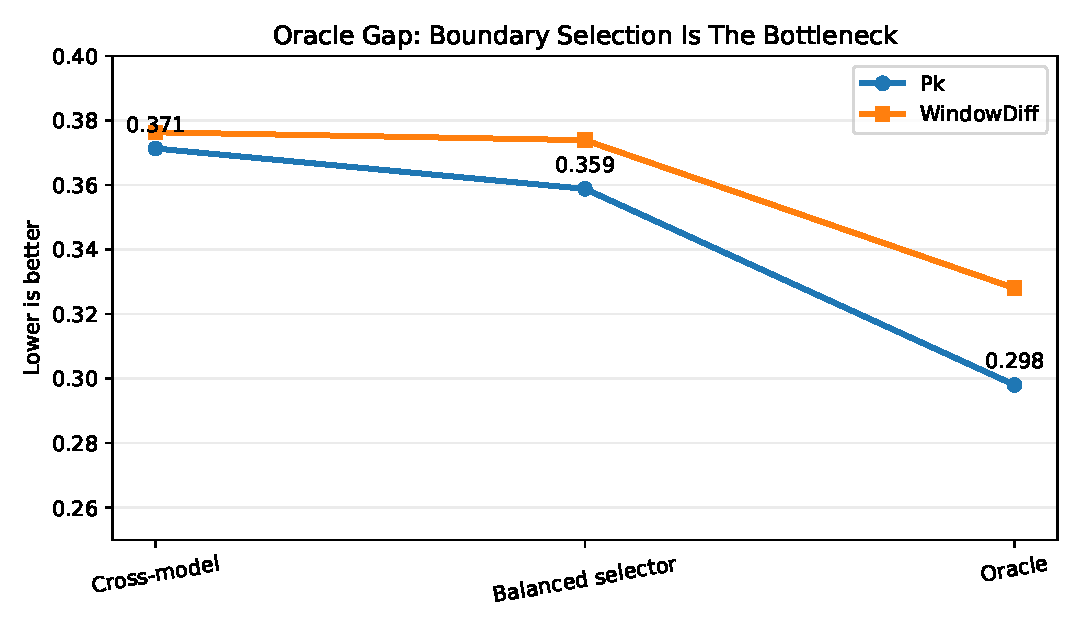
\includegraphics[width=0.82\linewidth]{figures/oracle_gap.pdf}
\end{frame}

\begin{frame}{Case Studies}
  \begin{itemize}
    \item Success: Physics videos where multimodal-grid variants reduce Pk/WD.
    \item Failure: selector over-switching damages Pk/WD on some videos.
    \item Domain weakness: Math needs better transcript/notation handling.
  \end{itemize}
  \vspace{0.5em}
  \small Evidence: \texttt{docs/CASE\_STUDIES.md}
\end{frame}

\begin{frame}{Compute Efficiency}
  \begin{itemize}
    \item Classical and cross-model methods run locally after embeddings are cached.
    \item Selector sweep is lightweight compared with training large chaptering models.
    \item High-resource systems use orders of magnitude more videos.
  \end{itemize}
\end{frame}

\begin{frame}{Limitations}
  \begin{itemize}
    \item 30-video seed benchmark, not a universal benchmark.
    \item Creator-provided chapters are useful but imperfect.
    \item Selector is not domain-general under leave-domain-out evaluation.
    \item Local LLM verifier is implemented but not promoted without full benchmark metrics.
  \end{itemize}
\end{frame}

\begin{frame}{Conclusion}
  \begin{itemize}
    \item LECSEG contributes a reproducible low-resource hierarchical lecture benchmark.
    \item It achieves statistically supported local gains over implemented baselines.
    \item The main research insight is the oracle gap: robust boundary selection remains unsolved.
  \end{itemize}
\end{frame}

\end{document}
